% Single-Source Shortest Paths -- Metropolis beamer slides
% Compile: pdflatex shortest-paths.tex (x2)
\documentclass[10pt,aspectratio=169]{beamer}

\usetheme{metropolis}
\metroset{block=fill, numbering=fraction, progressbar=frametitle}

\usepackage[T1]{fontenc}
\usepackage{amsmath, amssymb}
\usepackage{listings}
\usepackage{booktabs}
\usepackage{tikz}
\usetikzlibrary{arrows.meta, positioning, calc, decorations.pathmorphing}

% ---- colors -------------------------------------------------------------
\definecolor{mLightBlue}{HTML}{4C72B0}
\definecolor{mGreen}{HTML}{55A868}
\definecolor{mRed}{HTML}{C44E52}
\definecolor{mGray}{HTML}{BFBFBF}
\definecolor{mOrange}{HTML}{DD8452}
\setbeamercolor{alerted text}{fg=mRed}

% ---- code style ---------------------------------------------------------
\lstdefinestyle{jl}{
  basicstyle=\ttfamily\footnotesize,
  keywordstyle=\color{mRed}\bfseries,
  commentstyle=\color{mGreen}\itshape,
  numberstyle=\tiny\color{mGray},
  showstringspaces=false,
  breaklines=true,
  columns=fullflexible,
  morekeywords={function,for,in,if,else,elseif,end,return,length,while,continue,break}
}
\lstset{style=jl}

% ---- graph helpers ------------------------------------------------------
\tikzset{
  vtx/.style={draw, circle, minimum size=7mm, inner sep=0pt, font=\small,
              fill=white},
  edg/.style={thick, mGray!80!black},
  dedg/.style={edg, -{Stealth[length=2.5mm]}},
  hot/.style={line width=1.8pt, mLightBlue},
  wlbl/.style={fill=white, inner sep=1.5pt, font=\scriptsize, text=black},
  dlbl/.style={font=\scriptsize, inner sep=1pt},
  d0/.style={vtx, fill=mLightBlue!35},
  d1/.style={vtx, fill=mGreen!35},
  d2/.style={vtx, fill=mOrange!40},
  d3/.style={vtx, fill=mRed!30},
  cur/.style={vtx, fill=mOrange!45},
  fin/.style={vtx, fill=mGreen!35},
  tent/.style={vtx, fill=mLightBlue!20},
}

% ---- title --------------------------------------------------------------
\title{Single-Source Shortest Paths}
\subtitle{BFS, Dijkstra, Bellman-Ford}
\date{}
\author{}

\begin{document}

\maketitle

% =========================================================================
\begin{frame}{The Problem}
  Given a directed graph $G = (V, E)$ with edge weights $w(u, v)$ and a
  \alert{source} $s$, compute for every vertex $v$
  \[
    \text{dist}(s, v) = \text{the minimum total weight of a path from } s
    \text{ to } v.
  \]

  \pause
  \bigskip
  Which algorithm we use depends on the weights:

  \bigskip
  \begin{center}
  \begin{tabular}{llc}
    \toprule
    weights & algorithm & time \\
    \midrule
    all equal (unweighted) & BFS & $O(n + m)$ \\
    non-negative           & Dijkstra & $O((n + m) \log n)$ \\
    arbitrary, may be negative & Bellman-Ford & $O(nm)$ \\
    \bottomrule
  \end{tabular}
  \end{center}
\end{frame}

\begin{frame}{Shortest-Path Trees}
  \begin{block}{Optimal substructure}
    If a shortest path from $s$ to $v$ ends with the edge $u \to v$, then its
    prefix is a shortest path from $s$ to $u$.
  \end{block}

  \bigskip
  \begin{center}
  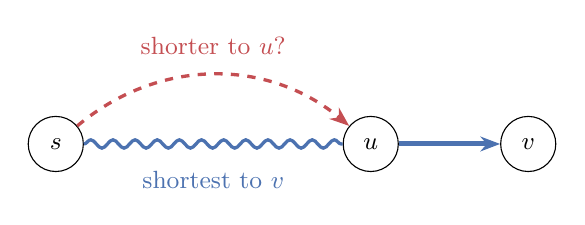
\begin{tikzpicture}[scale=1.0]
    \node[vtx] (s) at (0,0) {$s$};
    \node[vtx] (u) at (4,0) {$u$};
    \node[vtx] (v) at (6,0) {$v$};
    \draw[very thick, mLightBlue, decorate,
          decoration={snake, amplitude=1.5pt, segment length=8pt}] (s) -- (u);
    \draw[dedg, hot] (u) -- (v);
    \node[mLightBlue, font=\small] at (2,-0.45) {shortest to $v$};
    \onslide<2->{\draw[very thick, mRed, dashed, -{Stealth[length=2.5mm]}]
      (s) to[bend left=40] (u);
    \node[mRed, font=\small] at (2,1.25) {shorter to $u$?};}
  \end{tikzpicture}
  \end{center}

  \bigskip
  \onslide<2->{\begin{center}
    If the red path existed, red followed by $u \to v$ would beat the
    shortest path to $v$. Contradiction.
  \end{center}}
\end{frame}

\begin{frame}{Shortest-Path Trees}
  So each vertex only needs its \alert{parent}: the vertex just before it on a
  shortest path. The parent edges form a \alert{shortest-path tree} rooted
  at $s$.

  \bigskip
  \begin{columns}[c]
    \begin{column}{0.55\textwidth}
      \begin{center}
      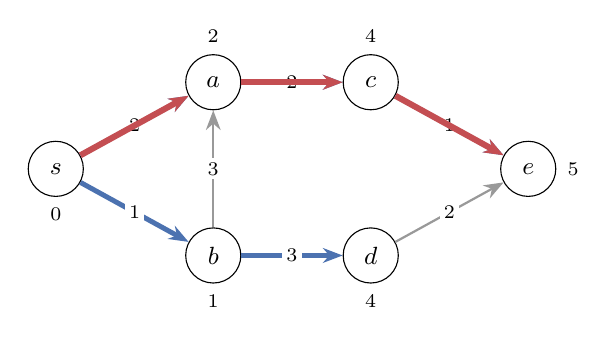
\begin{tikzpicture}[scale=1.0]
        \node[vtx] (s) at (0,0) {$s$};
        \node[vtx] (a) at (2,1.1) {$a$};  \node[vtx] (b) at (2,-1.1) {$b$};
        \node[vtx] (c) at (4,1.1) {$c$};  \node[vtx] (d) at (4,-1.1) {$d$};
        \node[vtx] (e) at (6,0) {$e$};
        \draw[dedg] (b) -- node[wlbl] {3} (a);
        \draw[dedg] (d) -- node[wlbl] {2} (e);
        \draw[dedg, hot] (s) -- node[wlbl] {2} (a);
        \draw[dedg, hot] (s) -- node[wlbl] {1} (b);
        \draw[dedg, hot] (a) -- node[wlbl] {2} (c);
        \draw[dedg, hot] (b) -- node[wlbl] {3} (d);
        \draw[dedg, hot] (c) -- node[wlbl] {1} (e);
        \only<2>{\draw[dedg, mRed, line width=2.2pt] (s) -- (a);
                 \draw[dedg, mRed, line width=2.2pt] (a) -- (c);
                 \draw[dedg, mRed, line width=2.2pt] (c) -- (e);}
        \node[dlbl, below=1mm of s] {$0$};
        \node[dlbl, above=1mm of a] {$2$};
        \node[dlbl, below=1mm of b] {$1$};
        \node[dlbl, above=1mm of c] {$4$};
        \node[dlbl, below=1mm of d] {$4$};
        \node[dlbl, right=1mm of e] {$5$};
      \end{tikzpicture}
      \end{center}
    \end{column}
    \begin{column}{0.42\textwidth}
      \small
      Small numbers are distances from $s$. Blue edges are the tree; $b \to a$
      and $d \to e$ are on no shortest path.

      \pause
      \bigskip
      Path to $e$: follow parents backwards,
      \[
        e \to c \to a \to s,
      \]
      so the shortest path is $s \to a \to c \to e$, of length $5$.
    \end{column}
  \end{columns}
\end{frame}

% =========================================================================
\section{BFS: Unweighted Graphs}

\begin{frame}{Breadth-First Search}
  Explore in \alert{waves}: every vertex at distance $d$ before any vertex at
  distance $d + 1$. A \alert{queue} (first in, first out) keeps the order.

  \bigskip
  \begin{center}
  \begin{tabular}{l}
    $\text{dist}[v] \gets \infty$ for all $v$; \ $\text{dist}[s] \gets 0$ \\
    $Q \gets [s]$ \\
    \textbf{while} $Q$ is not empty: \\
    \quad $u \gets$ dequeue$(Q)$ \\
    \quad \textbf{for} each neighbour $v$ of $u$: \\
    \quad\quad \textbf{if} $\text{dist}[v] = \infty$: \hfill \textit{first time we see $v$} \\
    \quad\quad\quad $\text{dist}[v] \gets \text{dist}[u] + 1$;
                    \ $\text{parent}[v] \gets u$ \\
    \quad\quad\quad enqueue$(Q, v)$
  \end{tabular}
  \end{center}
\end{frame}

% ---- BFS trace ----------------------------------------------------------
\begin{frame}{BFS in Action}
  BFS from $1$, neighbours in increasing order. Colour = distance.

  \bigskip
  \begin{columns}[c]
    \begin{column}{0.58\textwidth}
      \begin{center}
      \begin{tikzpicture}[scale=1.25]
        \coordinate (p1) at (0,1.5);    \coordinate (p2) at (1.5,1.5);
        \coordinate (p3) at (3,1.5);    \coordinate (p4) at (4.5,1.5);
        \coordinate (p5) at (0.75,0);   \coordinate (p6) at (2.25,0);
        \coordinate (p7) at (3.75,0);
        \foreach \i in {1,...,7} \node[vtx] (v\i) at (p\i) {\i};
        \foreach \a/\b in {1/2, 1/5, 2/3, 2/6, 3/4, 3/7, 5/6, 6/7}
          \draw[dedg] (v\a) -- (v\b);
        \draw[dedg] (v5) to[bend right=40] (v7);
        \only<2->{\draw[dedg, hot] (v1) -- (v2); \draw[dedg, hot] (v1) -- (v5);}
        \only<3->{\draw[dedg, hot] (v2) -- (v3); \draw[dedg, hot] (v2) -- (v6);}
        \only<4->{\draw[dedg, hot] (v5) to[bend right=40] (v7);}
        \only<5->{\draw[dedg, hot] (v3) -- (v4);}
        \node[d0] at (p1) {1};
        \only<2->{\node[d1] at (p2) {2}; \node[d1] at (p5) {5};}
        \only<3->{\node[d2] at (p3) {3}; \node[d2] at (p6) {6};}
        \only<4->{\node[d2] at (p7) {7};}
        \only<5->{\node[d3] at (p4) {4};}
      \end{tikzpicture}
      \end{center}
    \end{column}
    \begin{column}{0.4\textwidth}
      \small
      \only<1>{Start: $Q = [1]$, $\text{dist}[1] = 0$.}%
      \only<2>{Dequeue $1$: discover $2, 5$ at distance $1$.\\[4pt]
               $Q = [2, 5]$}%
      \only<3>{Dequeue $2$: discover $3, 6$ at distance $2$.\\[4pt]
               $Q = [5, 3, 6]$}%
      \only<4>{Dequeue $5$: $6$ is already seen; discover $7$ at
               distance $2$.\\[4pt] $Q = [3, 6, 7]$}%
      \only<5>{Dequeue $3$: discover $4$ at distance $3$; $7$ already
               seen.\\[4pt] $Q = [6, 7, 4]$}%
      \only<6>{Dequeue $6$, $7$, $4$: nothing new. $Q$ is empty.\\[6pt]
               \begin{tabular}{lccccccc}
                 $v$ & 1 & 2 & 3 & 4 & 5 & 6 & 7 \\
                 \midrule
                 dist & 0 & 1 & 2 & 3 & 1 & 2 & 2 \\
               \end{tabular}}
    \end{column}
  \end{columns}

  \bigskip
  \onslide<6>{\begin{center}\small Blue edges: the shortest-path tree.
  Edges $3 \to 7$, $5 \to 6$, $6 \to 7$ reach vertices already seen.
  \end{center}}
\end{frame}

\begin{frame}[fragile]{Reconstructing a Path}
  After BFS from $1$:
  \begin{center}
  \begin{tabular}{lccccccc}
    \toprule
    $v$ & 1 & 2 & 3 & 4 & 5 & 6 & 7 \\
    \midrule
    parent & -- & 1 & 2 & 3 & 1 & 2 & 5 \\
    \bottomrule
  \end{tabular}
  \end{center}

  \bigskip
  Path to $4$: \ $4 \xleftarrow{} 3 \xleftarrow{} 2 \xleftarrow{} 1$, so
  $1 \to 2 \to 3 \to 4$.

  \bigskip
\begin{lstlisting}
function reconstruct_path(parent, source, target)
    path = [target]
    while path[1] != source
        parent[path[1]] == 0 && return Int[]   # target unreachable
        pushfirst!(path, parent[path[1]])
    end
    return path
end
\end{lstlisting}
\end{frame}

\begin{frame}{Why BFS Is Correct}
  \begin{block}{Claim}
    For every $k \ge 0$: every vertex at distance $k$ from $s$ gets
    $\text{dist}[v] = k$, and all of them enter the queue after every vertex
    at distance $k - 1$ and before any vertex at distance $k + 1$.
  \end{block}

  \pause
  \bigskip
  \textbf{Induction on $k$.} For $k = 0$ only $s$ is enqueued, with label $0$.

  \bigskip
  Let $v$ be at distance $k + 1$, and let $u$ be the vertex before $v$ on a
  shortest path, so $u$ is at distance $k$.
  \begin{itemize}
    \item No vertex at distance $< k$ has an edge to $v$ (else
          $\text{dist}(s,v) \le k$), so $v$ is still unseen when the distance-$k$
          vertices start leaving the queue.
    \item When $u$ leaves the queue, $v$ is discovered, if not already, by a
          vertex at distance $k$, so $\text{dist}[v] = k + 1$.
  \end{itemize}
\end{frame}

\begin{frame}[fragile]{BFS: Running Time and Code}
  Each vertex is enqueued once and each list scanned once: $O(n + m)$.

\begin{lstlisting}[basicstyle=\ttfamily\scriptsize]
function bfs(n, adj, source)
    dist = fill(Inf, n)
    parent = zeros(Int, n)
    dist[source] = 0
    queue, head = Int[source], 1  # queue[head:end] is the live queue
    while head <= length(queue)
        u = queue[head]; head += 1
        for v in adj[u]
            if dist[v] == Inf
                dist[v] = dist[u] + 1
                parent[v] = u
                push!(queue, v)
            end
        end
    end
    return dist, parent
end
\end{lstlisting}
\end{frame}

% =========================================================================
\section{Dijkstra: Non-Negative Weights}

\begin{frame}{When Edges Have Weights}
  BFS minimises the \alert{number} of edges, not their total weight.

  \bigskip
  \begin{center}
  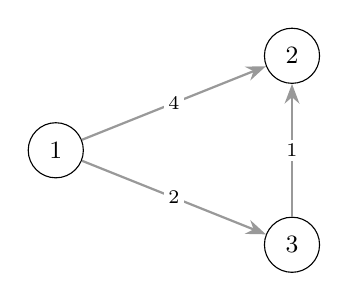
\begin{tikzpicture}[scale=1.0]
    \node[vtx] (1) at (0,0) {1}; \node[vtx] (2) at (3,1.2) {2};
    \node[vtx] (3) at (3,-1.2) {3};
    \draw[dedg] (1) -- node[wlbl] {4} (2);
    \draw[dedg] (1) -- node[wlbl] {2} (3);
    \draw[dedg] (3) -- node[wlbl] {1} (2);
  \end{tikzpicture}
  \end{center}

  \bigskip
  \begin{center}
    The direct edge $1 \to 2$ costs $4$, but $1 \to 3 \to 2$ costs only $3$.
  \end{center}
\end{frame}

\begin{frame}{Tense Edges and Relaxation}
  Keep a tentative distance $\text{dist}[v]$, always the length of
  \alert{some} path from $s$ to $v$ (or $\infty$).

  \bigskip
  An edge $u \to v$ is \alert{tense} if
  \[
    \text{dist}[u] + w(u, v) < \text{dist}[v]:
  \]
  going through $u$ is a shorter route to $v$ than the best one known.

  \pause
  \bigskip
  \alert{Relaxing} it fixes that:
  \[
    \text{dist}[v] \gets \text{dist}[u] + w(u, v), \qquad
    \text{parent}[v] \gets u.
  \]

  \bigskip
  \begin{center}
    Dijkstra and Bellman-Ford both just relax edges. They differ in
    \alert{which} edges and in \alert{what order}.
  \end{center}
\end{frame}

\begin{frame}{Dijkstra's Algorithm}
  Repeatedly \alert{finalise} the unfinished vertex with the smallest
  tentative distance, then relax its outgoing edges.

  \bigskip
  \begin{center}
  \begin{tabular}{l}
    $\text{dist}[v] \gets \infty$ for all $v$; \ $\text{dist}[s] \gets 0$ \\
    $R \gets V$ \hfill \textit{unfinished vertices} \\
    \textbf{while} $R$ is not empty: \\
    \quad $u \gets$ the vertex of $R$ with minimum $\text{dist}[u]$ \\
    \quad remove $u$ from $R$ \\
    \quad \textbf{for} each edge $u \to v$: \\
    \quad\quad \textbf{if} $\text{dist}[u] + w(u, v) < \text{dist}[v]$:
               \hfill \textit{tense} \\
    \quad\quad\quad $\text{dist}[v] \gets \text{dist}[u] + w(u, v)$;
                    \ $\text{parent}[v] \gets u$
  \end{tabular}
  \end{center}

  \bigskip
  \begin{center}
    \small BFS is the special case where every weight is $1$.
  \end{center}
\end{frame}

% ---- Dijkstra trace -----------------------------------------------------
\begin{frame}{Dijkstra in Action}
  \begin{columns}[c]
    \begin{column}{0.55\textwidth}
      \begin{center}
      \begin{tikzpicture}[scale=1.1]
        \coordinate (p1) at (0,0);   \coordinate (p2) at (3,1.2);
        \coordinate (p3) at (3,-1.2); \coordinate (p4) at (6,0);
        \foreach \i in {1,...,4} \node[vtx] (v\i) at (p\i) {\i};
        \draw[dedg] (v1) -- node[wlbl] {4} (v2);
        \draw[dedg] (v1) -- node[wlbl] {2} (v3);
        \draw[dedg] (v3) -- node[wlbl] {1} (v2);
        \draw[dedg] (v2) -- node[wlbl] {1} (v4);
        \draw[dedg] (v3) -- node[wlbl] {5} (v4);
        \only<2>{\draw[dedg, hot] (v1) -- (v2); \draw[dedg, hot] (v1) -- (v3);}
        \only<3>{\draw[dedg, hot] (v3) -- (v2); \draw[dedg, hot] (v3) -- (v4);}
        \only<4>{\draw[dedg, hot] (v2) -- (v4);}
        \only<5>{\draw[dedg, hot] (v1) -- (v3); \draw[dedg, hot] (v3) -- (v2);
                 \draw[dedg, hot] (v2) -- (v4);}
        % vertex states
        \only<1>{\node[tent] at (p1) {1};}
        \only<2>{\node[cur] at (p1) {1}; \node[tent] at (p2) {2};
                 \node[tent] at (p3) {3};}
        \only<3>{\node[fin] at (p1) {1}; \node[tent] at (p2) {2};
                 \node[cur] at (p3) {3}; \node[tent] at (p4) {4};}
        \only<4>{\node[fin] at (p1) {1}; \node[cur] at (p2) {2};
                 \node[fin] at (p3) {3}; \node[tent] at (p4) {4};}
        \only<5>{\node[fin] at (p1) {1}; \node[fin] at (p2) {2};
                 \node[fin] at (p3) {3}; \node[fin] at (p4) {4};}
        % distance labels
        \node[dlbl, below=1mm of v1] {$0$};
        \node[dlbl, above=1mm of v2]
          {\only<1>{$\infty$}\only<2>{$4$}\only<3->{$3$}};
        \node[dlbl, below=1mm of v3] {\only<1>{$\infty$}\only<2->{$2$}};
        \node[dlbl, right=1mm of v4]
          {\only<1-2>{$\infty$}\only<3>{$7$}\only<4->{$4$}};
      \end{tikzpicture}
      \end{center}
    \end{column}
    \begin{column}{0.42\textwidth}
      \small
      \only<1>{Initialise: $\text{dist}[1] = 0$, all others $\infty$.}%
      \only<2>{Extract $1$ ($0$). Relax $1 \to 2$: $4$. Relax $1 \to 3$: $2$.}%
      \only<3>{Extract $3$ ($2$). Relax $3 \to 2$: $\min(4, 2 + 1) = 3$.
               Relax $3 \to 4$: $7$.}%
      \only<4>{Extract $2$ ($3$). Relax $2 \to 4$: $\min(7, 3 + 1) = 4$.}%
      \only<5>{Extract $4$ ($4$). Done. Blue edges: the shortest-path tree.}

      \bigskip
      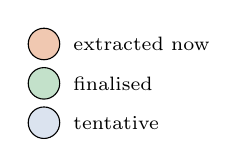
\begin{tikzpicture}[every node/.style={font=\scriptsize}]
        \node[cur, minimum size=4mm] at (0,0) {}; \node[right] at (0.25,0) {extracted now};
        \node[fin, minimum size=4mm] at (0,-0.5) {}; \node[right] at (0.25,-0.5) {finalised};
        \node[tent, minimum size=4mm] at (0,-1.0) {}; \node[right] at (0.25,-1.0) {tentative};
      \end{tikzpicture}
    \end{column}
  \end{columns}
\end{frame}

\begin{frame}{Correctness}
  \begin{block}{Invariant}
    When $u$ is removed from $R$, $\text{dist}[u] = \text{dist}(s, u)$.
  \end{block}

  \bigskip
  \textbf{Induction on the removal order.} $s$ goes first with
  $\text{dist}[s] = 0$. Now let $u$ be removed next with
  $\text{dist}[u] = d$, and suppose some path $P$ from $s$ to $u$ has length
  $d' < d$.

  \bigskip
  \begin{center}
  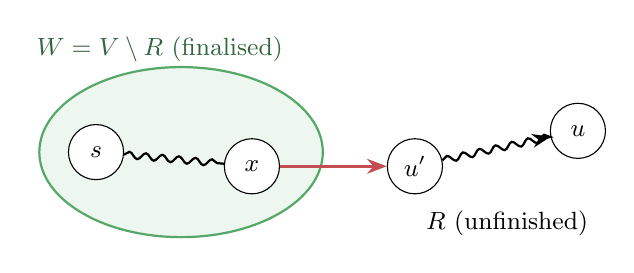
\begin{tikzpicture}[scale=0.9]
    \draw[mGreen, thick, fill=mGreen!10] (0.6,0) ellipse (2.0 and 1.2);
    \node[mGreen!60!black, font=\small] at (0.3,1.45) {$W = V \setminus R$ (finalised)};
    \node[vtx] (s) at (-0.6,0) {$s$};
    \node[vtx] (x) at (1.6,-0.2) {$x$};
    \node[vtx] (up) at (3.9,-0.2) {$u'$};
    \node[vtx] (u) at (6.2,0.3) {$u$};
    \draw[thick, decorate, decoration={snake, amplitude=1.2pt, segment length=6pt}]
      (s) -- (x);
    \draw[dedg, mRed, very thick] (x) -- (up);
    \draw[thick, decorate, decoration={snake, amplitude=1.2pt, segment length=6pt}, -{Stealth}]
      (up) -- (u);
    \node[font=\small] at (5.2,-1.0) {$R$ (unfinished)};
  \end{tikzpicture}
  \end{center}

  \small $P$ starts in $W$ and ends in $R$, so it has a first edge $x \to u'$
  with $x \in W$ and $u' \in R$.
\end{frame}

\begin{frame}{Correctness}
  $x$ is finalised, so by induction $\text{dist}[x] = \text{dist}(s, x)$,
  and edge $x \to u'$ was relaxed when $x$ was removed. Hence
  \[
    \text{dist}[u']
    \;\le\; \text{dist}[x] + w(x, u')
    \;\le\; \text{length of } P \text{ up to } u'
    \;\le\; d'
    \;<\; d,
  \]
  where the third step uses that the rest of $P$ has
  \alert{non-negative} weight.

  \pause
  \bigskip
  But Dijkstra removed $u$, not $u'$, so $d = \text{dist}[u] \le
  \text{dist}[u']$. Contradiction. $\square$
\end{frame}

\begin{frame}{Negative Edges Break It}
  \begin{columns}[c]
    \begin{column}{0.45\textwidth}
      \begin{center}
      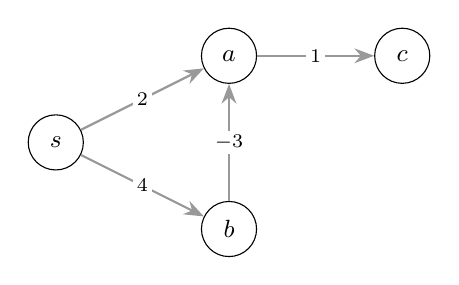
\begin{tikzpicture}[scale=1.0]
        \node[vtx] (s) at (0,0) {$s$};  \node[vtx] (a) at (2.2,1.1) {$a$};
        \node[vtx] (b) at (2.2,-1.1) {$b$}; \node[vtx] (c) at (4.4,1.1) {$c$};
        \draw[dedg] (s) -- node[wlbl] {2} (a);
        \draw[dedg] (s) -- node[wlbl] {4} (b);
        \draw[dedg] (b) -- node[wlbl] {$-3$} (a);
        \draw[dedg] (a) -- node[wlbl] {1} (c);
      \end{tikzpicture}
      \end{center}
    \end{column}
    \begin{column}{0.5\textwidth}
      \begin{itemize}
        \item Dijkstra finalises $s\ (0)$, $a\ (2)$, $c\ (3)$, then $b\ (4)$.
        \item Only then does it see $b \to a$: the true distance to $a$ is
              $4 - 3 = 1$.
        \item $c$ is already final with $3$, but $\text{dist}(s, c) = 2$.
      \end{itemize}
    \end{column}
  \end{columns}

  \bigskip
  \begin{center}
    The proof failed exactly where we used ``the rest of $P$ is
    non-negative''.
  \end{center}
\end{frame}

\begin{frame}{Running Time}
  \textbf{Linear scan for the minimum.} $n$ rounds, each scanning $R$ in
  $O(n)$, plus every edge relaxed once:
  \[
    O(n^2 + m).
  \]
  Good for \alert{dense} graphs.

  \pause
  \bigskip
  \textbf{Binary min-heap.} Push $(\text{dist}[v], v)$ on every relaxation,
  and skip \alert{stale} entries when popped. At most $m + 1$ pushes and pops,
  each $O(\log m) = O(\log n)$:
  \[
    O((n + m) \log n).
  \]
  Good for \alert{sparse} graphs.
\end{frame}

\begin{frame}[fragile]{Dijkstra in Julia}
\begin{lstlisting}[basicstyle=\ttfamily\scriptsize]
using DataStructures: PriorityQueue, enqueue!, dequeue_pair!

function dijkstra(n, adj, source)   # adj[u]: list of (v, weight) pairs
    dist   = fill(Inf, n)
    parent = zeros(Int, n)
    dist[source] = 0.0
    pq = PriorityQueue{Int, Float64}()
    enqueue!(pq, source, 0.0)
    while !isempty(pq)
        u, d = dequeue_pair!(pq)
        d > dist[u] && continue          # stale entry
        for (v, w) in adj[u]
            if dist[u] + w < dist[v]     # tense edge: relax it
                dist[v]   = dist[u] + w
                parent[v] = u
                pq[v] = dist[v]          # insert, or lower its key
            end
        end
    end
    return dist, parent
end
\end{lstlisting}
\end{frame}

% ---------------------------------------------------------------- exercise
\begin{frame}{Exercise}
  \begin{center}
    Run Dijkstra from $s$. Give the order in which vertices are finalised,
    the final distances, and the shortest-path tree.
  \end{center}

  \bigskip
  \begin{center}
  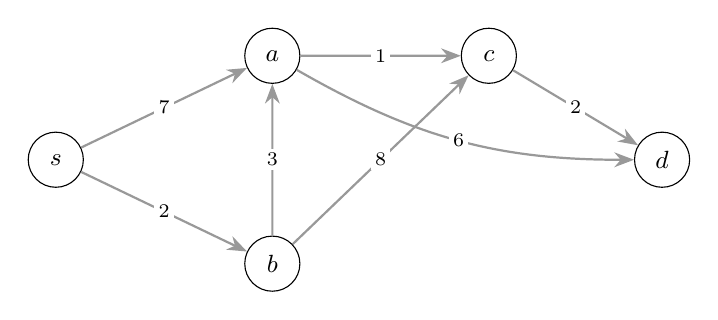
\begin{tikzpicture}[scale=1.1]
    \node[vtx] (s) at (0,0) {$s$};    \node[vtx] (a) at (2.5,1.2) {$a$};
    \node[vtx] (b) at (2.5,-1.2) {$b$}; \node[vtx] (c) at (5,1.2) {$c$};
    \node[vtx] (d) at (7,0) {$d$};
    \draw[dedg] (s) -- node[wlbl] {7} (a);
    \draw[dedg] (s) -- node[wlbl] {2} (b);
    \draw[dedg] (b) -- node[wlbl] {3} (a);
    \draw[dedg] (b) -- node[wlbl] {8} (c);
    \draw[dedg] (a) -- node[wlbl] {1} (c);
    \draw[dedg] (a) to[bend right=15] node[wlbl] {6} (d);
    \draw[dedg] (c) -- node[wlbl] {2} (d);
  \end{tikzpicture}
  \end{center}
\end{frame}

\begin{frame}{Solution}
  \begin{columns}[c]
    \begin{column}{0.48\textwidth}
      \small
      \begin{tabular}{lccccc}
        \toprule
        extract & $s$ & $a$ & $b$ & $c$ & $d$ \\
        \midrule
        start          & $0$ & $\infty$ & $\infty$ & $\infty$ & $\infty$ \\
        $s$ ($0$)      & & $7$ & $2$ & & \\
        $b$ ($2$)      & & $5$ & & $10$ & \\
        $a$ ($5$)      & & & & $6$ & $11$ \\
        $c$ ($6$)      & & & & & $8$ \\
        $d$ ($8$)      & & & & & \\
        \bottomrule
      \end{tabular}
    \end{column}
    \begin{column}{0.48\textwidth}
      \begin{center}
      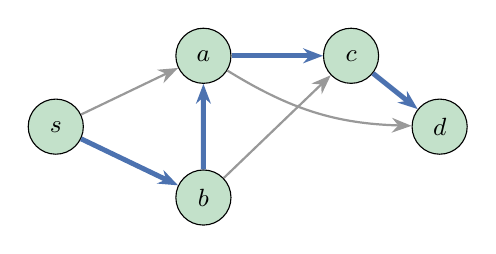
\begin{tikzpicture}[scale=0.75]
        \node[fin] (s) at (0,0) {$s$};    \node[fin] (a) at (2.5,1.2) {$a$};
        \node[fin] (b) at (2.5,-1.2) {$b$}; \node[fin] (c) at (5,1.2) {$c$};
        \node[fin] (d) at (6.5,0) {$d$};
        \draw[dedg] (s) -- (a); \draw[dedg] (b) -- (c);
        \draw[dedg] (a) to[bend right=15] (d);
        \draw[dedg, hot] (s) -- (b); \draw[dedg, hot] (b) -- (a);
        \draw[dedg, hot] (a) -- (c); \draw[dedg, hot] (c) -- (d);
      \end{tikzpicture}
      \end{center}
    \end{column}
  \end{columns}

  \bigskip
  \begin{center}
    Order $s, b, a, c, d$. \ Distances: $s{:}\,0$, $a{:}\,5$, $b{:}\,2$,
    $c{:}\,6$, $d{:}\,8$. \ Blue edges: the shortest-path tree.
  \end{center}
\end{frame}

% =========================================================================
\section{Bellman-Ford: Negative Weights}

\begin{frame}{Negative Edges and Negative Cycles}
  Negative weights are natural: rebates, energy gained, currency exchange
  with logarithms.

  \pause
  \bigskip
  But a \alert{negative cycle} reachable from $s$ makes distances
  meaningless: walk around it again and the total keeps falling.

  \bigskip
  \begin{center}
  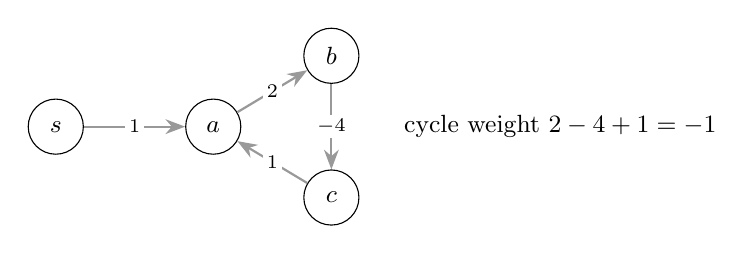
\begin{tikzpicture}[scale=1.0]
    \node[vtx] (s) at (0,0) {$s$};   \node[vtx] (a) at (2,0) {$a$};
    \node[vtx] (b) at (3.5,0.9) {$b$}; \node[vtx] (c) at (3.5,-0.9) {$c$};
    \draw[dedg] (s) -- node[wlbl] {1} (a);
    \draw[dedg] (a) -- node[wlbl] {2} (b);
    \draw[dedg] (b) -- node[wlbl] {$-4$} (c);
    \draw[dedg] (c) -- node[wlbl] {1} (a);
    \node[right, font=\small] at (4.3,0) {cycle weight $2 - 4 + 1 = -1$};
  \end{tikzpicture}
  \end{center}

  \pause
  \bigskip
  \textbf{Goal.} If no negative cycle is reachable from $s$, compute all
  distances. Otherwise, \alert{report} the negative cycle.
\end{frame}

\begin{frame}{The Key Fact}
  With no negative cycles, some shortest path to each $v$ is
  \alert{simple}: removing a cycle never makes a path longer.

  \bigskip
  A simple path visits at most $n$ vertices, so it uses
  \alert{at most $n - 1$ edges}.

  \pause
  \bigskip
  \begin{block}{Bellman-Ford}
    Relax \alert{every} edge, and repeat that $n - 1$ times.
  \end{block}

  \bigskip
  \begin{center}
    \small Round $k$ extends correct shortest paths by one more edge.
  \end{center}
\end{frame}

\begin{frame}{The Algorithm}
  \begin{center}
  \begin{tabular}{l}
    $\text{dist}[v] \gets \infty$ for all $v$; \ $\text{dist}[s] \gets 0$ \\
    \textbf{repeat} $n - 1$ times: \\
    \quad \textbf{for} each edge $u \to v$: \\
    \quad\quad \textbf{if} $\text{dist}[u] + w(u, v) < \text{dist}[v]$: \\
    \quad\quad\quad $\text{dist}[v] \gets \text{dist}[u] + w(u, v)$;
                    \ $\text{parent}[v] \gets u$ \\[6pt]
    \textbf{for} each edge $u \to v$: \hfill \textit{one more pass} \\
    \quad \textbf{if} $\text{dist}[u] + w(u, v) < \text{dist}[v]$: \\
    \quad\quad report ``negative cycle reachable from $s$''
  \end{tabular}
  \end{center}

  \bigskip
  \begin{center}
    $n - 1$ rounds of $m$ relaxations each: $O(nm)$.
  \end{center}
\end{frame}

% ---- Bellman-Ford trace -------------------------------------------------
\begin{frame}{Bellman-Ford in Action}
  Edges are scanned in the order $3 \to 4$, \ $2 \to 3$, \ $1 \to 2$, \
  $1 \to 4$ in every round.

  \bigskip
  \begin{columns}[c]
    \begin{column}{0.5\textwidth}
      \begin{center}
      \begin{tikzpicture}[scale=1.0]
        \coordinate (p1) at (0,0);   \coordinate (p2) at (2,1.2);
        \coordinate (p3) at (4,1.2); \coordinate (p4) at (6,0);
        \foreach \i in {1,...,4} \node[vtx] (v\i) at (p\i) {\i};
        \draw[dedg] (v1) -- node[wlbl] {2} (v2);
        \draw[dedg] (v2) -- node[wlbl] {$-4$} (v3);
        \draw[dedg] (v3) -- node[wlbl] {1} (v4);
        \draw[dedg] (v1) to[bend right=25] node[wlbl] {8} (v4);
        \only<2>{\draw[dedg, hot] (v1) -- (v2);
                 \draw[dedg, hot] (v1) to[bend right=25] (v4);}
        \only<3>{\draw[dedg, hot] (v2) -- (v3);}
        \only<4>{\draw[dedg, hot] (v3) -- (v4);}
        \node[dlbl, below=1mm of v1] {$0$};
        \node[dlbl, above=1mm of v2] {\only<1>{$\infty$}\only<2->{$2$}};
        \node[dlbl, above=1mm of v3] {\only<1-2>{$\infty$}\only<3->{$-2$}};
        \node[dlbl, below=1mm of v4]
          {\only<1>{$\infty$}\only<2-3>{$8$}\only<4->{$-1$}};
      \end{tikzpicture}
      \end{center}
    \end{column}
    \begin{column}{0.45\textwidth}
      \small
      \begin{tabular}{lcccc}
        \toprule
        after & 1 & 2 & 3 & 4 \\
        \midrule
        start & $0$ & $\infty$ & $\infty$ & $\infty$ \\
        \uncover<2->{round 1 & $0$ & $2$ & $\infty$ & $8$} \\
        \uncover<3->{round 2 & $0$ & $2$ & $-2$ & $8$} \\
        \uncover<4->{round 3 & $0$ & $2$ & $-2$ & $-1$} \\
        \bottomrule
      \end{tabular}
    \end{column}
  \end{columns}

  \bigskip
  \begin{center}
    \small
    \only<1>{$n = 4$, so $3$ rounds.}%
    \only<2>{Round 1: $3 \to 4$ and $2 \to 3$ start from $\infty$; then
             $1 \to 2$ and $1 \to 4$ fire.}%
    \only<3>{Round 2: $2 \to 3$ fires, $2 + (-4) = -2$.}%
    \only<4>{Round 3: $3 \to 4$ fires, $-2 + 1 = -1 < 8$. The path
             $1 \to 2 \to 3 \to 4$ beats the direct edge.}
  \end{center}
\end{frame}

\begin{frame}{Edge Order Matters, Rounds Don't}
  With the order $1 \to 2$, \ $2 \to 3$, \ $3 \to 4$, \ $1 \to 4$, a single
  round already gives the final answer $0, 2, -2, -1$.

  \bigskip
  \begin{itemize}
    \item A lucky order can finish early: stop as soon as a round changes
          nothing.
    \item An unlucky order needs all $n - 1$ rounds, which is what the
          analysis must cover.
  \end{itemize}

  \pause
  \bigskip
  \begin{center}
    The proof only uses one fact about a round: \alert{every} edge is relaxed
    at least once in it.
  \end{center}
\end{frame}

\begin{frame}{Correctness}
  \begin{block}{Claim}
    After round $k$, $\text{dist}[v] \le$ the weight of the shortest path
    from $s$ to $v$ that uses at most $k$ edges.
  \end{block}

  \bigskip
  \textbf{Induction on $k$.} Round $0$: $\text{dist}[s] = 0$, everything
  else $\infty$.

  \bigskip
  Round $k$: take the best path $P$ to $v$ with at most $k$ edges, and let
  $u \to v$ be its last edge. The rest of $P$ uses at most $k - 1$ edges,
  so after round $k - 1$, $\text{dist}[u] \le w(P) - w(u, v)$. Relaxing
  $u \to v$ in round $k$ gives
  \[
    \text{dist}[v] \;\le\; \text{dist}[u] + w(u, v) \;\le\; w(P).
  \]

  \pause
  \textbf{So after $n - 1$ rounds:} $\text{dist}[v] \le \text{dist}(s, v)$
  by the key fact, and $\text{dist}[v] \ge \text{dist}(s, v)$ since it is
  always the weight of some path. They are equal. $\square$
\end{frame}

\begin{frame}{Detecting Negative Cycles}
  \begin{block}{Claim}
    After $n - 1$ rounds, some edge is still tense $\iff$ a negative cycle is
    reachable from $s$.
  \end{block}

  \bigskip
  (tense $\Rightarrow$ cycle) Suppose no negative cycle is reachable. Then
  the distances are exact, and exact distances satisfy
  $\text{dist}(s, v) \le \text{dist}(s, u) + w(u, v)$, so nothing is tense.

  \pause
  \bigskip
  (cycle $\Rightarrow$ tense) Let $v_1 \to \cdots \to v_k \to v_1$ be a reachable
  negative cycle (all its $\text{dist}$ values are finite). If no edge were
  tense, then $\text{dist}[v_{i+1}] \le \text{dist}[v_i] + w(v_i, v_{i+1})$
  around the whole cycle. Adding these up, the $\text{dist}$ terms cancel:
  \[
    0 \;\le\; \sum_{\text{cycle}} w(v_i, v_{i+1}) \;<\; 0.
  \]
  Contradiction. $\square$
\end{frame}

\begin{frame}[fragile]{Bellman-Ford in Julia}
  \begin{columns}[T]
    \begin{column}{0.56\textwidth}
\begin{lstlisting}[basicstyle=\ttfamily\scriptsize]
function bellman_ford(n, adj, source)
    # adj[u] is a list of (v, weight) pairs
    dist   = fill(Inf, n)
    parent = zeros(Int, n)
    dist[source] = 0.0
    for _ in 1:n-1
        updated = false
        for u in 1:n
            dist[u] == Inf && continue
            for (v, w) in adj[u]
                if dist[u] + w < dist[v]
                    dist[v]   = dist[u] + w
                    parent[v] = u
                    updated   = true
                end
            end
        end
        updated || break   # already final
    end
\end{lstlisting}
    \end{column}
    \begin{column}{0.42\textwidth}
\begin{lstlisting}[basicstyle=\ttfamily\scriptsize]
    # one more pass
    for u in 1:n
        for (v, w) in adj[u]
            if dist[u] + w < dist[v]
                error("negative cycle")
            end
        end
    end
    return dist, parent
end
\end{lstlisting}

      \bigskip
      \small The early exit keeps the worst case at $O(nm)$ but often stops
      much sooner.
    \end{column}
  \end{columns}
\end{frame}

% =========================================================================
\begin{frame}{Summary}
  \begin{center}
  \begin{tabular}{llll}
    \toprule
    algorithm & weights & idea & time \\
    \midrule
    BFS & unweighted & waves, a queue & $O(n + m)$ \\
    Dijkstra & $\ge 0$ & finalise the closest unfinished vertex
             & $O((n + m) \log n)$ \\
    Bellman-Ford & any & relax every edge, $n - 1$ times & $O(nm)$ \\
    \bottomrule
  \end{tabular}
  \end{center}

  \bigskip
  \begin{itemize}
    \item All three build a shortest-path tree through parent pointers.
    \item Dijkstra and Bellman-Ford are both sequences of relaxations of tense
          edges.
    \item Use the fastest algorithm the weights allow.
  \end{itemize}
\end{frame}

\end{document}
